% Generated layout for figures/make_aregion_figures.py panels (rendering only; see VERIFY_AREGION.json).
\definecolor{okgreen}{RGB}{0,158,115}\definecolor{okorange}{RGB}{230,159,0}
\definecolor{okblue}{RGB}{0,114,178}\definecolor{okgrey}{RGB}{238,238,238}
\begin{figure}[htbp]
\centering
\setlength{\tabcolsep}{1.5pt}
\begin{tabular}{@{}ccccc@{}}
 & $s_{\text{card}}=10^{-4}$ & $s_{\text{card}}=10^{-2}$ & $s_{\text{card}}=10^{0}$ & $s_{\text{card}}=10^{2}$ \\
\rotatebox{90}{\small\ stage2\_01} & 
\includegraphics[width=0.19\linewidth]{figures/panels/stage2_01_card00.png} & 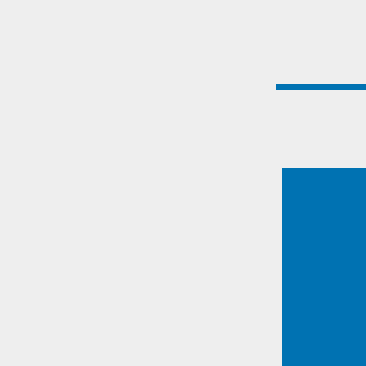
\includegraphics[width=0.19\linewidth]{figures/panels/stage2_01_card20.png} & 
\includegraphics[width=0.19\linewidth]{figures/panels/stage2_01_card40.png} & 
\includegraphics[width=0.19\linewidth]{figures/panels/stage2_01_card60.png} \\[1pt]
\rotatebox{90}{\small\ stage2\_02} & 
\includegraphics[width=0.19\linewidth]{figures/panels/stage2_02_card00.png} & 
\includegraphics[width=0.19\linewidth]{figures/panels/stage2_02_card20.png} & 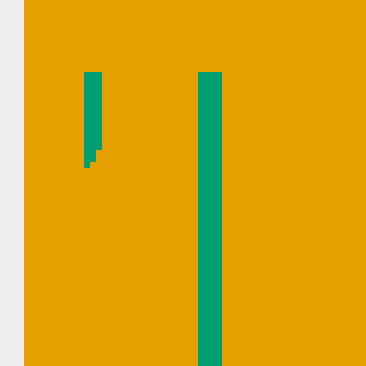
\includegraphics[width=0.19\linewidth]{figures/panels/stage2_02_card40.png} & 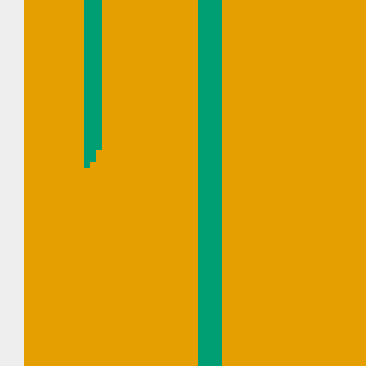
\includegraphics[width=0.19\linewidth]{figures/panels/stage2_02_card60.png} \\[1pt]
\rotatebox{90}{\small\ stage2\_03} & 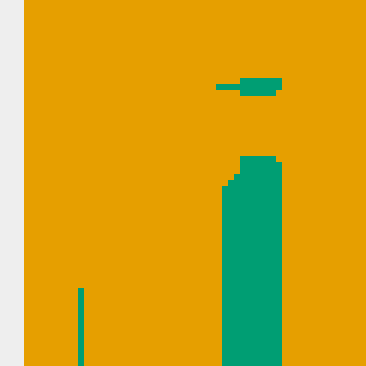
\includegraphics[width=0.19\linewidth]{figures/panels/stage2_03_card00.png} & 
\includegraphics[width=0.19\linewidth]{figures/panels/stage2_03_card20.png} & 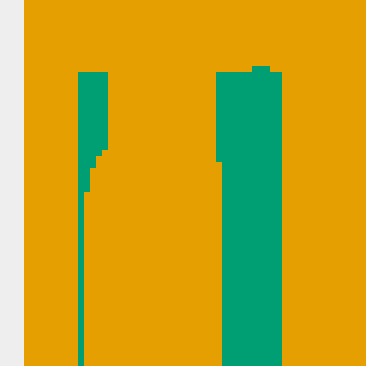
\includegraphics[width=0.19\linewidth]{figures/panels/stage2_03_card40.png} & 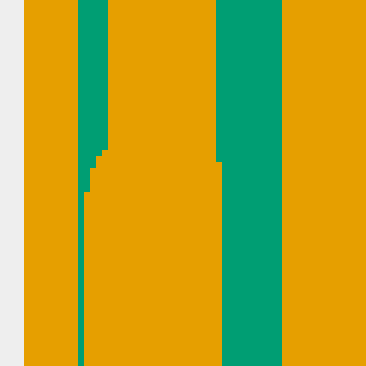
\includegraphics[width=0.19\linewidth]{figures/panels/stage2_03_card60.png} \\[1pt]
\rotatebox{90}{\small\ stage2\_04} & 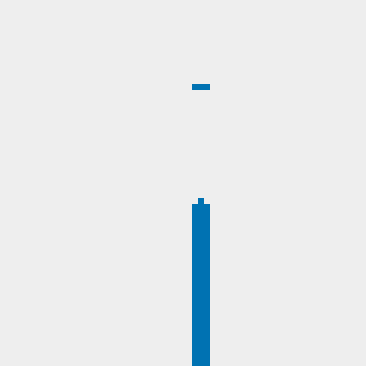
\includegraphics[width=0.19\linewidth]{figures/panels/stage2_04_card00.png} & 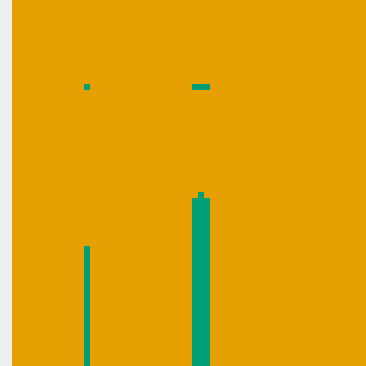
\includegraphics[width=0.19\linewidth]{figures/panels/stage2_04_card20.png} & 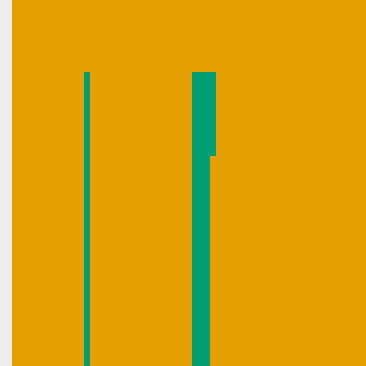
\includegraphics[width=0.19\linewidth]{figures/panels/stage2_04_card40.png} & 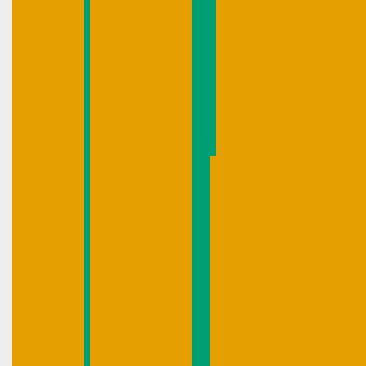
\includegraphics[width=0.19\linewidth]{figures/panels/stage2_04_card60.png} \\[1pt]
\rotatebox{90}{\small\ stage2\_05} & 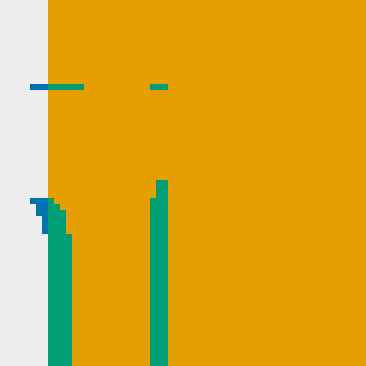
\includegraphics[width=0.19\linewidth]{figures/panels/stage2_05_card00.png} & 
\includegraphics[width=0.19\linewidth]{figures/panels/stage2_05_card20.png} & 
\includegraphics[width=0.19\linewidth]{figures/panels/stage2_05_card40.png} & 
\includegraphics[width=0.19\linewidth]{figures/panels/stage2_05_card60.png} \\[1pt]
\end{tabular}

\smallskip
{\small
\fcolorbox{black!40}{okgreen}{\rule{0pt}{4pt}\rule{4pt}{0pt}}~A for both encodings\quad
\fcolorbox{black!40}{okorange}{\rule{0pt}{4pt}\rule{4pt}{0pt}}~A for slack only\quad
\fcolorbox{black!40}{okblue}{\rule{0pt}{4pt}\rule{4pt}{0pt}}~A for unbalanced only\quad
\fcolorbox{black!40}{okgrey}{\rule{0pt}{4pt}\rule{4pt}{0pt}}~A for neither}
\caption{Stage-2 A-regions at the primary matching parameter $r=1$. Each row is one
instance and each column one slice of the cardinality axis (every twentieth grid
value, fixed before plotting). Within a panel, $s_{\text{budget}}$ increases to the
right and $s_{\text{sector}}$ upward, each over the full grid from $10^{-4}$ to
$10^{2}$; each square is one grid point coloured by its exact labels, with nothing
fitted or smoothed. Full-grid label counts reproduce Table~\ref{tab:reader-stage2}.\dag}
\label{fig:aregions}
\end{figure}
